% Chapter Template

\chapter{Model Architecture and Training}

\label{Chapter4}

\section{Model structure}
The structure of the neural network is such that it contains some number $n$ of fully connected layers and batch normalization for each layer, along with regularization. All of these layers have the same number of units. The last layer has a dropout of 50\%. In addition to these layers there is one more output layer. This is simply a dense layer with 1 unit. A grid search was performed to determine the hyperparameters that minimize the loss. Hyperparameters are parameters that are set before the training begins\cite{hyperparameters_definition}. These hyperparameters include number of units in each layer, number of epochs to train for, number of layers, batch size, optimizer and penalty to enforce in the regularization. The possible combinations tried can be seen in Table \ref{table:gridSearchHyperparamters}.

\begin{table}[h]
    \centering
    \caption[Hyperparameter search with best performing combination.]{Hyperparamter search with best performing combination shown. Hyperparameter search was done using hyperband algorithm that initially searches randomly for the best parameters but then hones in on what is working and as such is neither exhaustive nor completely random. This means that a hard upper limit will not be set on the number of combinations to try like with randomsearch.}
    \label{table:gridSearchHyperparamters}
    \begin{tabular}{ccc}
        \toprule
        Parameter & Range of values & Selected\\
        \midrule
        Layers &  min\_value = 4, max\_value = 15, step = 1 & \textbf{10}\\
        Units &  min\_value = 32, max\_value = 512, step = 32 & \textbf{64}\\
        Penalties & min\_value = 1e-5, max\_value = 1, sampling = log & \textbf{1e-4}\\
        Epochs & min\_value = 10, max\_value = 1000, step = 10 & \textbf{250}\\
        Optimizers & Adam, RMSprop, Adamax & \textbf{Adamax}\\
        Activation & ReLU, ELu, Softmax & \textbf{ReLU}\\
        \bottomrule
    \end{tabular}
\end{table}

As mentioned, hyperband doesn't set a hard upper limit to the number of epochs it will train in total. When using the \href{https://keras.io/api/keras_tuner/tuners/hyperband/}{hyperband class} several factors can be set. One of interest here is the $hyperband_iterations$ argument. This determines how often the hyperband algorithm is run and defaults to 1. For each iteration the epochs are distributed between tries (that is each set of hyperparameters) with the total amount of epochs approximately $n_{epochs} = max_{epochs} * log^2(max_{epochs})\approx 10^4$, where $max_{epochs} = 1000$ gives the maximum number of epochs that one set of hyperparameters can be trained for. Searching a space generally takes a lot of time but this drastically improves on gridsearch. If each epoch takes around 10 seconds to run then the total search would take around 28 hours on a shared resource. This is resource intensive and cannot be repeated often. Another question that remains is whether the ranges given are optimal. Are a 1000 epochs even enough?

\section{Model Training}
To determine the required number of epochs a high number of epochs can be selected and the loss plotted. These plots can be seen in Figures (\ref{fig:loss_plot_wo_elevation}, \ref{fig:loss_plot_w_elevation}). Looking at these two plots, training loss decreases for over 1900 epochs in both plots, while the validation loss stops decreasing at around 200 epochs for DEM model and 1800 epochs for model without DEM. This is unexpected. The DEM model has vastly more parameters and as such should contain more useful information to be learned, which one might expect to take longer to learn. This does not seem to be the case. The DEM model only gets trivially better after 1000 epochs while the non DEM model keeps meaningfully improving until around 1800 epochs. With respect to time constraints of shared resources models were trained for 250 epochs.

\begin{figure}
    \centering
    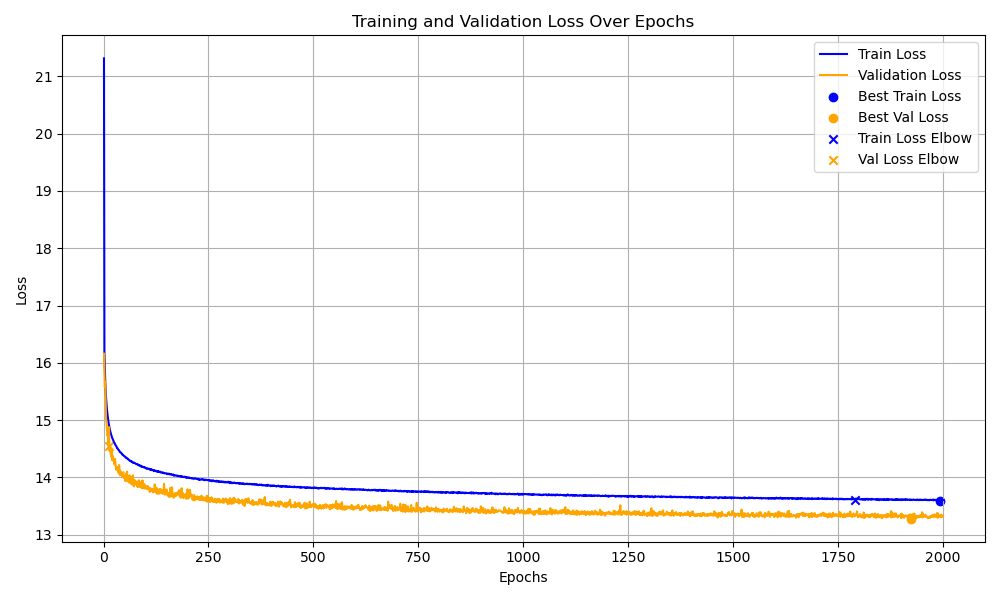
\includegraphics[scale = 0.6]{Figures/loss_plot_wo_elevation.png}
    \caption[Loss plot of model trained for 2000 without DEM.]{Loss plot of model trained for 2000 without DEM.}
    \label{fig:loss_plot_wo_elevation}
\end{figure}


\begin{figure}
    \centering
    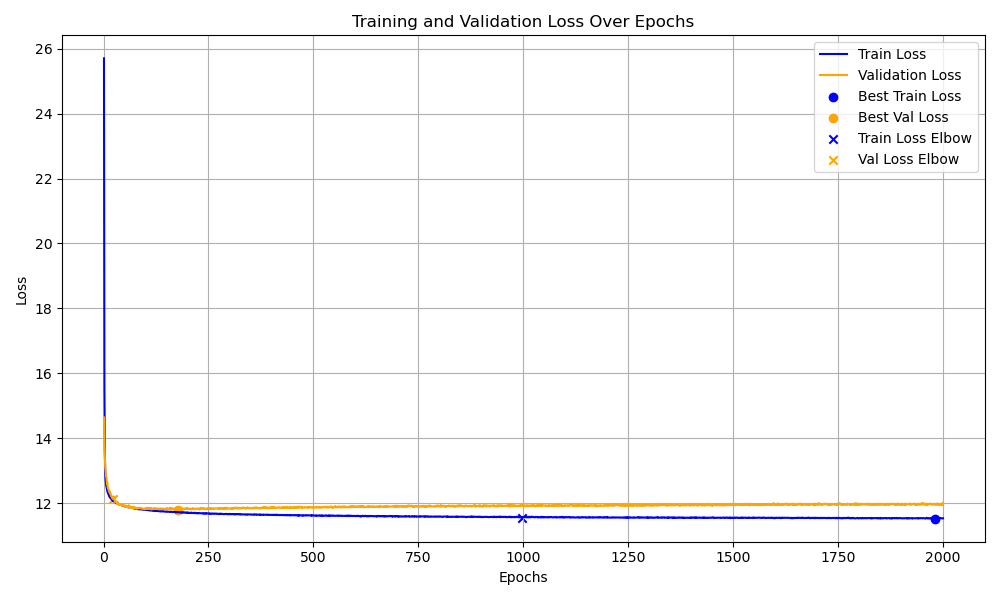
\includegraphics[scale = 0.6]{Figures/loss_plot_w_elevation.png}
    \caption[Loss plot of model trained for 2000 with DEM.]{Loss plot of model trained for 2000 with DEM.}
    \label{fig:loss_plot_w_elevation}
\end{figure}